\documentclass[10pt]{article}
% \def\StudentVersion{}
\usepackage{../../common}
\makeatletter

\def\LecStr{Alexander Rush}
\def\LecNum{1}
\def\LecTitle{Lectures Notes on Search}
\def\LecDate{}

\def\Graph{\path node(A)[draw, initial, state] at (-2, 1) {A};
    \path node(B)[draw, state] at (-1, 3) {B};
    \path node(C)[draw, state, accepting] at (4, 2) {C};
    \path node(D)[draw, state] at (1, 1) {D};
    \path node(E)[draw, state] at (2, 3) {E};
    \path[draw] (A) --node[xshift=-0.2cm]{2} (B); 
    \path[draw] (B) --node[yshift=0.2cm]{4} (E); 
    \path[draw] (A) --node[yshift=0.2cm]{3} (D); 
    \path[draw] (A) --node[yshift=0.2cm]{5} (E); 
    \path[draw] (D) --node[yshift=0.2cm]{4} (C); 
    \path[draw] (E) --node[yshift=0.2cm]{4} (C); 
}

\def\Words{
  \matrix(dict)[matrix of nodes, ampersand replacement=\&]{
    Mary \& golpeo \& la \& bruja \& verde \\
    ~\\
    ~\\
    Mary \& slapped \& the \& green \& witch \\ };
}

\begin{document}
\MakeScribeTop{}

\section{Board 0}

- Start with XKCD (have it on when they come in)

- Show pacman searches

\section{Board 0}

\begin{itemize}
\item Homework extension Monday at midnight (HW questions)
\item Section Lyman 425
\item Laptop policy
\item name tags...
\end{itemize}

\section{board 0.5}
\begin{itemize}
\item mistake $n$ depth $n+1$
\item Depth $m$ 
\end{itemize}

\section{Board 1}
\begin{itemize}
\item Completeness; Is the algorithm guaranteed to find a solution? (infinite paths)
\item Optimality; Is the algorithm guaranteed to find the optimal solution?
\item Time:
\item Space:
\end{itemize}

\section{Board 2}

Redraw table:

\begin{table}
  \centering
  \begin{tabular}{llll}
    
    DFS &  \\
    BFS &  \\
    Depth Limited &  \\
    Iterative Deepening & \\
  \end{tabular}
\end{table}

\section{Board 3}

Summary

\begin{itemize}
\item Algorithms
\begin{itemize}
\item Uniform-Cost Search 
\end{itemize}
\item Heuristics
\item Informed Search
  \begin{itemize}
  \item Greedy Best-First Search 
  \item A* Search
  \end{itemize}
\end{itemize}


\section{Board 4}

Uniform-cost search

Idea: Fix BFS optimality

\begin{itemize}
\item Be conservative based on path-cost (as opposed to depth)
\item Expand in path cost order
\item Utilize a priority queue
\end{itemize}

Priority function: \[f:\mcP \mapsto \reals^+\]

\section{Board 5}

Recall 

$c$ is step cost 

$g$ is path cost


For UCS, we set this
function to be $f(p)\triangleq g(p)$, i.e. the cost of the partial
path.

% The failure case for the optimality of BFS is when there is a deep
% node that has a lower cost than a shallower node. BFS fails to be
% optimal in this case, because it order paths by depth. Uniform-cost
% Search (UCS) fixes this issue by ordering paths by cost instead. 

% To do this we use a \textbf{priority queue} where 'pop' gives the next
% path based on a priority function. Define the priority function as:
% $f:\mcP \mapsto \reals$ to select the next path. 

\section{Board 6}

\begin{center}
\begin{tabular}{ccccll}
  \toprule
  iter & $p$ & $f$ & $s$ & frontier ($p$) & explored \\
  \midrule
  0 & - & & - & \censor{[A:0]} & \censor{\{\}} \\
  1 &A & 0 & A & \censor{[A:B:2, A:D:3, A:E:5]} & \censor{\{A\}} \\
  2 &A:B & 2 & B & \censor{[A:D:3, A:E:5]} & \censor{\{A, B\}} \\
  3 &A:D & 3 & D  & \censor{[A:E:5, A:D:C:7] }& \censor{\{A, B, D\}} \\
  4 &A:E & 5 & E & \censor{[A:D:C:8]} & \censor{\{A, B, D, E\}} \\
  5 &A:D:C & C & 8 & - & - \\
  \bottomrule
\end{tabular}
\end{center}


Because UCS expands paths in cost order and costs are non-negative,
each path it expands must be at least as costly as all previous paths.
This means that if UCS finds a goal node it must be optimal. With a few 
further assumptions (see AIMA) we can also show it is complete. AIMA also 
includes a description of the time- and space-complexity that uses 
the optimal score and smallest path cost $\epsilon$. 

\section{Board 7}

\begin{itemize}
\item Completeness: Yes.  
\item Optimality: Yes.
\item Time-Complexity: $O(b^{1 + \lfloor C^*/\delta \rfloor } )$  (smallest step cost)
\item Space-Complexity: $O(b^{1 + \lfloor C^*/\delta \rfloor } )$ 
\end{itemize}


\section{Board 8}

Uninformed vs. Informed



Up to this point we assumed that we have no further knowledge into the
nature of the search model. With this requirement there is no hope to
find an optimal solution without first expanding all path with cost $<
C*$ (as in UCS).  However it in practice we often have more insight
into the structure of the problem, for instance roughly how close we 
are to a goal state. When we have this information we can instead run 
informed search.


\section{Board 9}

Heuristic: Guess at future cost.

- number of dots left
- best translation for each word
- shortest line cost
\begin{center}
\begin{tabularx}{\linewidth}{llX}
  \toprule \\
 Heuristic & $h: \mcS \mapsto \reals$ & Estimate of cost from state $s$ to a goal state. \\\\
\bottomrule
\end{tabularx}
\end{center}


\section{Board 10}


\begin{figure}
  \centering

  \begin{tikzpicture}
    \Graph
    \draw[dashed,red] (A)--node[yshift=0.2cm]{6} (C); 
    \draw[dashed,red] (B)--node[yshift=-0.2cm]{6} (C); 
  \end{tikzpicture}

 
  \caption{\label{fig:heu} An example heuristic: straight-line distance.}
\end{figure}

\section{Board 11}

\textbf{Greedy Best-First Search}

\begin{itemize}
\item Be greedy on heuristic! 
\item Expand in heuristic cost order
\item 
\end{itemize}

Same setup as UCS but with 
 \[f(p) = h(p_{\mathrm{Last}}) \]  


\section{Board 12} 

\begin{itemize}
\item Completeness: No.  
\item Optimality: No. 
\item Time-Complexity: $O(b^m)$
\item Space-Complexity: $O(b^m)$ 
\end{itemize}

\section{Board 13}

- Combine UCS and Greedy Best-first

\[f(p) \triangleq g(p) + h(p_{\mathrm{Last}}) \]  

- A* search. 


\section{14}

\begin{center}
\begin{tabular}{cccll}
  \toprule
  iter & $p$ & $s$ & frontier ($p$) & explored \\
  \midrule
  0 & - & - & \censor{[A=0+6]} & \censor{\{\}} \\
  1 &A & A & \censor{[ A:D=3+4, A:B=2+6, A:E=5+4]} & \censor{\{A\}} \\
  2 &A:D & D & \censor{[A:D:C:7+0, A:B=2+6, A:E=5+4]} & \censor{\{A, D\}} \\
  3 &A:D:C & C  & -& - \\
  \bottomrule
\end{tabular}
\end{center}

\section{Board 14} 

\begin{itemize}
\item Completeness: Yes.  
\item Optimality: ?. 
% \item Time-Complexity: $O(b^m)$
% \item Space-Complexity: $O(b^m)$ 
\end{itemize}

\section{Board 14.5}
Let $p$ be $(s_0, a_0), \ldots, (s_{n-1}, a_{n-1})$
  
Define a (strict) subpath of $p \in \mcP$ as $(s_0, a_0), \ldots, (s_{n'-1}, a_{n'-1})$
for $n' \leq n$.

By our definition of cost $g(p') \leq g(p)$.


\section{Board 15}

\begin{defn}
  An \textbf{admissible} heuristic never overestimates the cost to a goal state, i.e.  \[g(p) +
  h(p_{\mathrm{Last}}) \leq g(\hat{p})\] where $\hat{p}\in \mcQ$ is any solution with 
  $p$ as a sub-path.
\end{defn}

\begin{defn}
  A  \textbf{consistent} heuristic obeys the property that for any state $s$, \[h(s) \leq c(s, a)
  + h(\msc{Res}(s, a))\]
 for all
  actions $a \in \msc{Act}(s)$.
\end{defn}

Consistency $\Rightarrow$ admissibility. However, there are cases where just admissibility is sufficient so we define both.


% We first prove that the A$^*$ estimated cost increase at each expansion, and then use this to show that the first expansion of any state is optimal. This implies that the first time we expand a goal state is optimal.  

\section{Board 16}

\begin{theorem}
  $A^*$  with consistent heuristic is optimal.
\end{theorem}

\noindent \textbf{Proof:}


\textbf{The values of expanded paths are non-decreasing.}

Assume expansion of path $p$ leads to $p'$ with action $a$:

\begin{eqnarray*}
f(p') &=& g(p') + h(p_{\mathrm{Last}}') = g(p) + c(p_{\mathrm{last}}, a) + h(p'_{\mathrm{last}})  \\
&\geq & g(p) + h(p_{\mathrm{Last}}) =f(p),
\end{eqnarray*}

\noindent Where we have directly used the definition of consistency for the inequality.

\section{Board 17}

\textbf{ After $A^*$ expands a path, the optimal path to that state has already been expanded. }

By contradiction.

Assume we have expand path $p \in \mcP$ before the optimal path to this state $q \in \mcP$. 

\air 
Implies $p_{\mathrm{last}} =q_\mathrm{last}$ and  $g(q) < g(p)$, this implies $f(q) < f(p)$.
\air

Since we expanded $p$ first, this also mean there is some sub-path
of $q$ (called $q'$) in frontier.
\air


 Also we know that $f(p) \leq f(q')$ (or else it would have been expanded first).

\air

However by Property~(1) we know that as a sub-path of $q$, $f(q') \leq f(q)$. 
\air 

Together this gives a contradiction:

\ifthenelse{\isundefined{\StudentVersion}}{
\censor{}
\[ f(q) < f(p) \leq f(q') \leq f(q) \] 
}{
\vspace{1cm}
\censor{}

}


\QED

% \noindent Property~(2) implies that whenever $A^*$ expands the goal state it must be the optimal path to the goal.

\section{Board 18}
\begin{itemize}
\item Completeness: Yes.  (graph-search requires both, tree-search just need admissable)
\item Optimality: Yes. 
\item Time-Complexity: $O(b^\Delta)$ (depends on the absolute error of $h$, see AIMA3e, p.98)
\item Memory-Complexity: $O(b^\Delta)$ (graph search)
\end{itemize}


\section{Board 19}
\subsection{Heuristics for Path-Finding}

Now let's return to the heuristics we discussed above. How can we check whether they satisfy the properties necessary for A$^*$ search? First consider straight-line distance. We would like to show that for any state $s$ and valid action $a$:

\[h(s) \leq c(s, a) + h(\msc{Res}(s, a))\]

\noindent and let's call the resulting state $s' = \msc{Res}(s, a)$.

We have defined our problem such that the cost of the action is the distance between $s$ and $s'$, i.e. $d(s, s')$. And we have defined our heuristic $h(s)$ as the distance to our goal $h(s) = d(s, \mathrm{C})$. So for consistency we need to show that: 



\[d(s, \mathrm{C}) \leq d(s, s') + d(s', \mathrm{C})\]

\noindent However this is just the triangle inequality! Since this holds for Euclidean distance, we have consistency for this problem.


% \section{Board 21}

% Traveling Salesman Problem

% Story time. 

\section{Board 20}

\subsection{Comparing Heuristic Functions}

\[\Delta(p, s) = g(\hat{p}^*) - (g(p) + h(p_{\mathrm{Last}})) \] 

\begin{defn}
  Given two consistent heuristics $h$ and $h'$, we say $h$ \textbf{dominates} $h'$ if 
  for all $s\in\mcS$, $h(s) \geq h'(s)$. 
\end{defn}

\section{Board 21}

\begin{itemize}
\item Write down the explicit constraints that are required for the problem. 
\item Select a subset of these constraints to ``relax''.
\item Calculate the optimal solution without these constraints and use as heuristic.   
\end{itemize}

% Oftentimes when the constraints are dropped the problem becomes much more efficient to solve, and it leads to an admissible heuristic since we are making it strictly easier to reach any goal.

% For path-finding we relaxed the problem by assuming we did not have to follow any of the paths directly. This allows get an underestimate of the solution. For translation, our problem assumed that each word was translated exactly once. Our heuristic is to relax this constraint and allow any remaining word translated multiple times. We can compute this heuristic cost very efficiently, and it gives us an underestimate of the optimal. 


taking $h(s) = \max\{ h_1(s), h_2(s)\}$.

% While all consistent heuristics will find an optimal solution, not all
% consistent heuristics are equal. As you will discover first hand in
% the homework, a better heuristic will find the optimal solution much
% quicker, and in fact the time and memory complexity of A$*$ depend on 
% the quality of the heuristic. A better heuristic will produce a smaller
% absolute error $\delta$, where delta is the difference from the completing 
% path $\hat{p}^*$.


% We can use this to compare different heuristics. Basically we would like 
% the heuristic that produces the highest estimate while still maintaining 
% consistency.


% In the simplest case, if we have two heuristics $h_1$ and $h_2$, we
% can construct an admissible heuristic that is at least as good by
% taking $h(s) = \max\{ h_1(s), h_2(s)\}$.

% \begin{exercise}
%   Show that this heuristic $h$ is still admissible.
% \end{exercise}
    
% In section we will further explore various.

% \subsection{Generating Heuristic Functions}

% A harder question though is how to generate consistent heuristics for arbitrary problems. How do we come up with heuristic for real problems? And how do we show that they satisfy consistency? 

% One method for doing is known as \textbf{relaxation}. Generally the approach works like this:

% \begin{itemize}
% \item Write down the explicit constraints that are required for the problem. 
% \item Select a subset of these constraints to ``relax''.
% \item Calculate the optimal solution without these constraints and use as heuristic.   
% \end{itemize}

% Oftentimes when the constraints are dropped the problem becomes much more efficient to solve, and it leads to an admissible heuristic since we are making it strictly easier to reach any goal.

% For path-finding we relaxed the problem by assuming we did not have to follow any of the paths directly. This allows get an underestimate of the solution. For translation, our problem assumed that each word was translated exactly once. Our heuristic is to relax this constraint and allow any remaining word translated multiple times. We can compute this heuristic cost very efficiently, and it gives us an underestimate of the optimal. 




% \subsection{Relaxation Example: 8-Puzzle}

% In practice, coming up with good relaxations is the key for finding efficient, optimal search algorithms. In your homework, you will construct various heuristics for difficult maze problems. To help with this, in section, we will go over examples of relaxations. In particular we will look at the various heuristics developed for the 8-Puzzle problem below: 

% \begin{center}
%   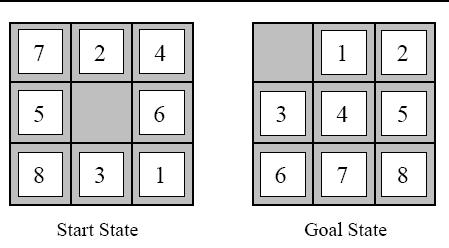
\includegraphics{pics/puzzle}
% \end{center}

% % If we are clever this heuristic cost can be made very efficient by precomputing values. 

% % AIMA gives several more examples of effective heuristic for difficult search problems.

\end{document}
